%%%%%%%%%%%%%%%%%%%%%%%%%%%%%%%%%%%%%%%%%
% The Legrand Orange Book
% LaTeX Template
% Version 1.4 (12/4/14)
%
% This template has been downloaded from:
% http://www.LaTeXTemplates.com
%
% Original author:
% Mathias Legrand (legrand.mathias@gmail.com)
% 
% Modified by:
% Andy Ridgwell (andy@seao2.org)
%
% License:
% CC BY-NC-SA 3.0 (http://creativecommons.org/licenses/by-nc-sa/3.0/)
%
% Compiling this template:
% This template uses biber for its bibliography and makeindex for its index.
% When you first open the template, compile it from the command line with the 
% commands below to make sure your LaTeX distribution is configured correctly:
%
% 1) pdflatex main
% 2) makeindex main.idx -s StyleInd.ist
% 3) biber main
% 4) pdflatex main x 2
%
% After this, when you wish to update the bibliography/index use the appropriate
% command above and make sure to compile with pdflatex several times 
% afterwards to propagate your changes to the document.
%
% This template also uses a number of packages which may need to be
% updated to the newest versions for the template to compile. It is strongly
% recommended you update your LaTeX distribution if you have any
% compilation errors.
%
% Important note:
% Chapter heading images should have a 2:1 width:height ratio,
% e.g. 920px width and 460px height.
%
%%%%%%%%%%%%%%%%%%%%%%%%%%%%%%%%%%%%%%%%%

%----------------------------------------------------------------------------------------
%       PACKAGES AND OTHER DOCUMENT CONFIGURATIONS
%----------------------------------------------------------------------------------------

\documentclass[11pt,fleqn]{book} % Default font size and left-justified equations

\usepackage[top=3.0cm,bottom=3cm,left=3.2cm,right=3.2cm,headsep=10pt,letterpaper]{geometry} % Page margins

\usepackage{xcolor} % Required for specifying colors by name
\definecolor{ocre}{RGB}{243,102,25} % Define the orange color used for highlighting throughout the book

% Font Settings
\usepackage{avant} % Use the Avantgarde font for headings
%\usepackage{times} % Use the Times font for headings
\usepackage{mathptmx} % Use the Adobe Times Roman as the default text font together with math symbols from the Sym­bol, Chancery and Com­puter Modern fonts

\usepackage{microtype} % Slightly tweak font spacing for aesthetics
\usepackage[utf8]{inputenc} % Required for including letters with accents
\usepackage[T1]{fontenc} % Use 8-bit encoding that has 256 glyphs

% Index
\usepackage{calc} % For simpler calculation - used for spacing the index letter headings correctly
\usepackage{makeidx} % Required to make an index
\makeindex % Tells LaTeX to create the files required for indexing

%----------------------------------------------------------------------------------------

%----------------------------------------------------------------------------------------
%	VARIOUS REQUIRED PACKAGES
%----------------------------------------------------------------------------------------

\usepackage{titlesec} % Allows customization of titles

\usepackage{graphicx} % Required for including pictures
\graphicspath{{graphics/}} % Specifies the directory where pictures are stored

\usepackage{lipsum} % Inserts dummy text

\usepackage{tikz} % Required for drawing custom shapes

\usepackage[english]{babel} % English language/hyphenation

\usepackage{enumitem} % Customize lists
\setlist{nolistsep} % Reduce spacing between bullet points and numbered lists

\usepackage{booktabs} % Required for nicer horizontal rules in tables

\usepackage{eso-pic} % Required for specifying an image background in the title page

%----------------------------------------------------------------------------------------
%	MAIN TABLE OF CONTENTS
%----------------------------------------------------------------------------------------

\usepackage{titletoc} % Required for manipulating the table of contents

\contentsmargin{0cm} % Removes the default margin
% Chapter text styling
\titlecontents{chapter}[1.25cm] % Indentation
{\addvspace{15pt}\large\sffamily\bfseries} % Spacing and font options for chapters
{\color{ocre!60}\contentslabel[\Large\thecontentslabel]{1.25cm}\color{ocre}} % Chapter number
{}  
{\color{ocre!60}\normalsize\sffamily\bfseries\;\titlerule*[.5pc]{.}\;\thecontentspage} % Page number
% Section text styling
\titlecontents{section}[1.25cm] % Indentation
{\addvspace{5pt}\sffamily\bfseries} % Spacing and font options for sections
{\contentslabel[\thecontentslabel]{1.25cm}} % Section number
{}
{\sffamily\hfill\color{black}\thecontentspage} % Page number
[]
% Subsection text styling
\titlecontents{subsection}[1.25cm] % Indentation
{\addvspace{1pt}\sffamily\small} % Spacing and font options for subsections
{\contentslabel[\thecontentslabel]{1.25cm}} % Subsection number
{}
{\sffamily\;\titlerule*[.5pc]{.}\;\thecontentspage} % Page number
[] 

%----------------------------------------------------------------------------------------
%	MINI TABLE OF CONTENTS IN CHAPTER HEADS
%----------------------------------------------------------------------------------------

% Section text styling
\titlecontents{lsection}[0em] % Indendating
{\footnotesize\sffamily} % Font settings
{}
{}
{}

% Subsection text styling
\titlecontents{lsubsection}[.5em] % Indentation
{\normalfont\footnotesize\sffamily} % Font settings
{}
{}
{}
 
%----------------------------------------------------------------------------------------
%	PAGE HEADERS
%----------------------------------------------------------------------------------------

\usepackage{fancyhdr} % Required for header and footer configuration

\pagestyle{fancy}
\renewcommand{\chaptermark}[1]{\markboth{\sffamily\normalsize\bfseries\chaptername\ \thechapter.\ #1}{}} % Chapter text font settings
\renewcommand{\sectionmark}[1]{\markright{\sffamily\normalsize\thesection\hspace{5pt}#1}{}} % Section text font settings
\fancyhf{} \fancyhead[LE,RO]{\sffamily\normalsize\thepage} % Font setting for the page number in the header
\fancyhead[LO]{\rightmark} % Print the nearest section name on the left side of odd pages
\fancyhead[RE]{\leftmark} % Print the current chapter name on the right side of even pages
\renewcommand{\headrulewidth}{0.5pt} % Width of the rule under the header
\addtolength{\headheight}{2.5pt} % Increase the spacing around the header slightly
\renewcommand{\footrulewidth}{0pt} % Removes the rule in the footer
\fancypagestyle{plain}{\fancyhead{}\renewcommand{\headrulewidth}{0pt}} % Style for when a plain pagestyle is specified

% Removes the header from odd empty pages at the end of chapters
\makeatletter
\renewcommand{\cleardoublepage}{
\clearpage\ifodd\c@page\else
\hbox{}
\vspace*{\fill}
\thispagestyle{empty}
\newpage
\fi}

%----------------------------------------------------------------------------------------
%	THEOREM STYLES
%----------------------------------------------------------------------------------------

\usepackage{amsmath,amsfonts,amssymb,amsthm} % For math equations, theorems, symbols, etc

\newcommand{\intoo}[2]{\mathopen{]}#1\,;#2\mathclose{[}}
\newcommand{\ud}{\mathop{\mathrm{{}d}}\mathopen{}}
\newcommand{\intff}[2]{\mathopen{[}#1\,;#2\mathclose{]}}
\newtheorem{notation}{Notation}[chapter]

%%%%%%%%%%%%%%%%%%%%%%%%%%%%%%%%%%%%%%%%%%%%%%%%%%%%%%%%%%%%%%%%%%%%%%%%%%%
%%%%%%%%%%%%%%%%%%%% dedicated to boxed/framed environements %%%%%%%%%%%%%%
%%%%%%%%%%%%%%%%%%%%%%%%%%%%%%%%%%%%%%%%%%%%%%%%%%%%%%%%%%%%%%%%%%%%%%%%%%%
\newtheoremstyle{ocrenumbox}% % Theorem style name
{0pt}% Space above
{0pt}% Space below
{\normalfont}% % Body font
{}% Indent amount
{\small\bf\sffamily\color{ocre}}% % Theorem head font
{\;}% Punctuation after theorem head
{0.25em}% Space after theorem head
{\small\sffamily\color{ocre}\thmname{#1}\nobreakspace\thmnumber{\@ifnotempty{#1}{}\@upn{#2}}% Theorem text (e.g. Theorem 2.1)
\thmnote{\nobreakspace\the\thm@notefont\sffamily\bfseries\color{black}---\nobreakspace#3.}} % Optional theorem note
\renewcommand{\qedsymbol}{$\blacksquare$}% Optional qed square

\newtheoremstyle{blacknumex}% Theorem style name
{5pt}% Space above
{5pt}% Space below
{\normalfont}% Body font
{} % Indent amount
{\small\bf\sffamily}% Theorem head font
{\;}% Punctuation after theorem head
{0.25em}% Space after theorem head
{\small\sffamily{\tiny\ensuremath{\blacksquare}}\nobreakspace\thmname{#1}\nobreakspace\thmnumber{\@ifnotempty{#1}{}\@upn{#2}}% Theorem text (e.g. Theorem 2.1)
\thmnote{\nobreakspace\the\thm@notefont\sffamily\bfseries---\nobreakspace#3.}}% Optional theorem note

\newtheoremstyle{blacknumbox} % Theorem style name
{0pt}% Space above
{0pt}% Space below
{\normalfont}% Body font
{}% Indent amount
{\small\bf\sffamily}% Theorem head font
{\;}% Punctuation after theorem head
{0.25em}% Space after theorem head
{\small\sffamily\thmname{#1}\nobreakspace\thmnumber{\@ifnotempty{#1}{}\@upn{#2}}% Theorem text (e.g. Theorem 2.1)
\thmnote{\nobreakspace\the\thm@notefont\sffamily\bfseries---\nobreakspace#3.}}% Optional theorem note

%%%%%%%%%%%%%%%%%%%%%%%%%%%%%%%%%%%%%%%%%%%%%%%%%%%%%%%%%%%%%%%%%%%%%%%%%%%
%%%%%%%%%%%%% dedicated to non-boxed/non-framed environements %%%%%%%%%%%%%
%%%%%%%%%%%%%%%%%%%%%%%%%%%%%%%%%%%%%%%%%%%%%%%%%%%%%%%%%%%%%%%%%%%%%%%%%%%
\newtheoremstyle{ocrenum}% % Theorem style name
{5pt}% Space above
{5pt}% Space below
{\normalfont}% % Body font
{}% Indent amount
{\small\bf\sffamily\color{ocre}}% % Theorem head font
{\;}% Punctuation after theorem head
{0.25em}% Space after theorem head
{\small\sffamily\color{ocre}\thmname{#1}\nobreakspace\thmnumber{\@ifnotempty{#1}{}\@upn{#2}}% Theorem text (e.g. Theorem 2.1)
\thmnote{\nobreakspace\the\thm@notefont\sffamily\bfseries\color{black}---\nobreakspace#3.}} % Optional theorem note
\renewcommand{\qedsymbol}{$\blacksquare$}% Optional qed square
\makeatother

% Defines the theorem text style for each type of theorem to one of the three styles above
\newcounter{dummy} 
\numberwithin{dummy}{section}
\theoremstyle{ocrenumbox}
\newtheorem{theoremeT}[dummy]{Theorem}
\newtheorem{problem}{Problem}[chapter]
\newtheorem{exerciseT}{Exercise}[chapter]
\theoremstyle{blacknumex}
\newtheorem{exampleT}{Example}[chapter]
\theoremstyle{blacknumbox}
\newtheorem{vocabulary}{Vocabulary}[chapter]
\newtheorem{definitionT}{Definition}[section]
\newtheorem{corollaryT}[dummy]{Corollary}
\theoremstyle{ocrenum}
\newtheorem{proposition}[dummy]{Proposition}

%----------------------------------------------------------------------------------------
%	DEFINITION OF COLORED BOXES
%----------------------------------------------------------------------------------------

\RequirePackage[framemethod=default]{mdframed} % Required for creating the theorem, definition, exercise and corollary boxes

% Theorem box
\newmdenv[skipabove=7pt,
skipbelow=7pt,
backgroundcolor=black!5,
linecolor=ocre,
innerleftmargin=5pt,
innerrightmargin=5pt,
innertopmargin=5pt,
leftmargin=0cm,
rightmargin=0cm,
innerbottommargin=5pt]{tBox}

% Exercise box	  
\newmdenv[skipabove=7pt,
skipbelow=7pt,
rightline=false,
leftline=true,
topline=false,
bottomline=false,
backgroundcolor=ocre!10,
linecolor=ocre,
innerleftmargin=5pt,
innerrightmargin=5pt,
innertopmargin=5pt,
innerbottommargin=5pt,
leftmargin=0cm,
rightmargin=0cm,
linewidth=4pt]{eBox}	

% Definition box
\newmdenv[skipabove=7pt,
skipbelow=7pt,
rightline=false,
leftline=true,
topline=false,
bottomline=false,
linecolor=ocre,
innerleftmargin=5pt,
innerrightmargin=5pt,
innertopmargin=0pt,
leftmargin=0cm,
rightmargin=0cm,
linewidth=4pt,
innerbottommargin=0pt]{dBox}	

% Corollary box
\newmdenv[skipabove=7pt,
skipbelow=7pt,
rightline=false,
leftline=true,
topline=false,
bottomline=false,
linecolor=gray,
backgroundcolor=black!5,
innerleftmargin=5pt,
innerrightmargin=5pt,
innertopmargin=5pt,
leftmargin=0cm,
rightmargin=0cm,
linewidth=4pt,
innerbottommargin=5pt]{cBox}

% Creates an environment for each type of theorem and assigns it a theorem text style from the "Theorem Styles" section above and a colored box from above
\newenvironment{theorem}{\begin{tBox}\begin{theoremeT}}{\end{theoremeT}\end{tBox}}
\newenvironment{exercise}{\begin{eBox}\begin{exerciseT}}{\hfill{\color{ocre}\tiny\ensuremath{\blacksquare}}\end{exerciseT}\end{eBox}}				  
\newenvironment{definition}{\begin{dBox}\begin{definitionT}}{\end{definitionT}\end{dBox}}	
\newenvironment{example}{\begin{exampleT}}{\hfill{\tiny\ensuremath{\blacksquare}}\end{exampleT}}		
\newenvironment{corollary}{\begin{cBox}\begin{corollaryT}}{\end{corollaryT}\end{cBox}}	

%----------------------------------------------------------------------------------------
%	REMARK ENVIRONMENT
%----------------------------------------------------------------------------------------

\newenvironment{remark}{\par\vspace{10pt}\small % Vertical white space above the remark and smaller font size
\begin{list}{}{
\leftmargin=35pt % Indentation on the left
\rightmargin=25pt}\item\ignorespaces % Indentation on the right
\makebox[-2.5pt]{\begin{tikzpicture}[overlay]
\node[draw=ocre!60,line width=1pt,circle,fill=ocre!25,font=\sffamily\bfseries,inner sep=2pt,outer sep=0pt] at (-15pt,0pt){\textcolor{ocre}{R}};\end{tikzpicture}} % Orange R in a circle
\advance\baselineskip -1pt}{\end{list}\vskip5pt} % Tighter line spacing and white space after remark

%----------------------------------------------------------------------------------------
%	SECTION NUMBERING IN THE MARGIN
%----------------------------------------------------------------------------------------

\makeatletter
\renewcommand{\@seccntformat}[1]{\llap{\textcolor{ocre}{\csname the#1\endcsname}\hspace{1em}}}                    
\renewcommand{\section}{\@startsection{section}{1}{\z@}
{-4ex \@plus -1ex \@minus -.4ex}
{1ex \@plus.2ex }
{\normalfont\large\sffamily\bfseries}}
\renewcommand{\subsection}{\@startsection {subsection}{2}{\z@}
{-3ex \@plus -0.1ex \@minus -.4ex}
{0.5ex \@plus.2ex }
{\normalfont\sffamily\bfseries}}
\renewcommand{\subsubsection}{\@startsection {subsubsection}{3}{\z@}
{-2ex \@plus -0.1ex \@minus -.2ex}
{.2ex \@plus.2ex }
{\normalfont\small\sffamily\bfseries}}                        
\renewcommand\paragraph{\@startsection{paragraph}{4}{\z@}
{-2ex \@plus-.2ex \@minus .2ex}
{.1ex}
{\normalfont\small\sffamily\bfseries}}

%----------------------------------------------------------------------------------------
%	HYPERLINKS IN THE DOCUMENTS
%----------------------------------------------------------------------------------------

% For an unclear reason, the package should be loaded now and not later
\usepackage{hyperref}
\hypersetup{hidelinks,backref=true,pagebackref=true,hyperindex=true,colorlinks=false,breaklinks=true,urlcolor= ocre,bookmarks=true,bookmarksopen=false,pdftitle={Title},pdfauthor={Author}}

%----------------------------------------------------------------------------------------
%	CHAPTER HEADINGS
%----------------------------------------------------------------------------------------

% The set-up below should be (sadly) manually adapted to the overall margin page septup controlled by the geometry package loaded in the main.tex document. It is possible to implement below the dimensions used in the goemetry package (top,bottom,left,right)... TO BE DONE

\newcommand{\thechapterimage}{}
\newcommand{\chapterimage}[1]{\renewcommand{\thechapterimage}{#1}}

% Numbered chapters with mini tableofcontents
\def\thechapter{\arabic{chapter}}
\def\@makechapterhead#1{
\thispagestyle{empty}
{\centering \normalfont\sffamily
\ifnum \c@secnumdepth >\m@ne
\if@mainmatter
\startcontents
\begin{tikzpicture}[remember picture,overlay]
\node at (current page.north west)
{\begin{tikzpicture}[remember picture,overlay]
\node[anchor=north west,inner sep=0pt] at (0,0) {\includegraphics[width=\paperwidth]{\thechapterimage}};
%%%%%%%%%%%%%%%%%%%%%%%%%%%%%%%%%%%%%%%%%%%%%%%%%%%%%%%%%%%%%%%%%%%%%%%%%%%%%%%%%%%%%
% Commenting the 3 lines below removes the small contents box in the chapter heading
\fill[color=ocre!10!white,opacity=.6] (1cm,0) rectangle (8cm,-7cm);
\node[anchor=north west] at (1.1cm,.35cm) {\parbox[t][8cm][t]{6.5cm}{\huge\bfseries\flushleft \printcontents{l}{1}{\setcounter{tocdepth}{2}}}};
\draw[anchor=west] (5cm,-9cm) node [rounded corners=20pt,fill=ocre!10!white,text opacity=1,draw=ocre,draw opacity=1,line width=1.5pt,fill opacity=.6,inner sep=12pt]{\huge\sffamily\bfseries\textcolor{black}{\thechapter. #1\strut\makebox[22cm]{}}};
%%%%%%%%%%%%%%%%%%%%%%%%%%%%%%%%%%%%%%%%%%%%%%%%%%%%%%%%%%%%%%%%%%%%%%%%%%%%%%%%%%%%%
\end{tikzpicture}};
\end{tikzpicture}}
\par\vspace*{230\p@}
\fi
\fi}

% Unnumbered chapters without mini tableofcontents (could be added though) 
\def\@makeschapterhead#1{
\thispagestyle{empty}
{\centering \normalfont\sffamily
\ifnum \c@secnumdepth >\m@ne
\if@mainmatter
\begin{tikzpicture}[remember picture,overlay]
\node at (current page.north west)
{\begin{tikzpicture}[remember picture,overlay]
\node[anchor=north west,inner sep=0pt] at (0,0) {\includegraphics[width=\paperwidth]{\thechapterimage}};
\draw[anchor=west] (5cm,-9cm) node [rounded corners=20pt,fill=ocre!10!white,fill opacity=.6,inner sep=12pt,text opacity=1,draw=ocre,draw opacity=1,line width=1.5pt]{\huge\sffamily\bfseries\textcolor{black}{#1\strut\makebox[22cm]{}}};
\end{tikzpicture}};
\end{tikzpicture}}
\par\vspace*{230\p@}
\fi
\fi
}
\makeatother % Insert the commands.tex file which contains the majority of the structure behind the template

\begin{document}

%----------------------------------------------------------------------------------------
%       TITLE PAGE
%----------------------------------------------------------------------------------------

\begingroup
\thispagestyle{empty}
\AddToShipoutPicture*{\put(0,0){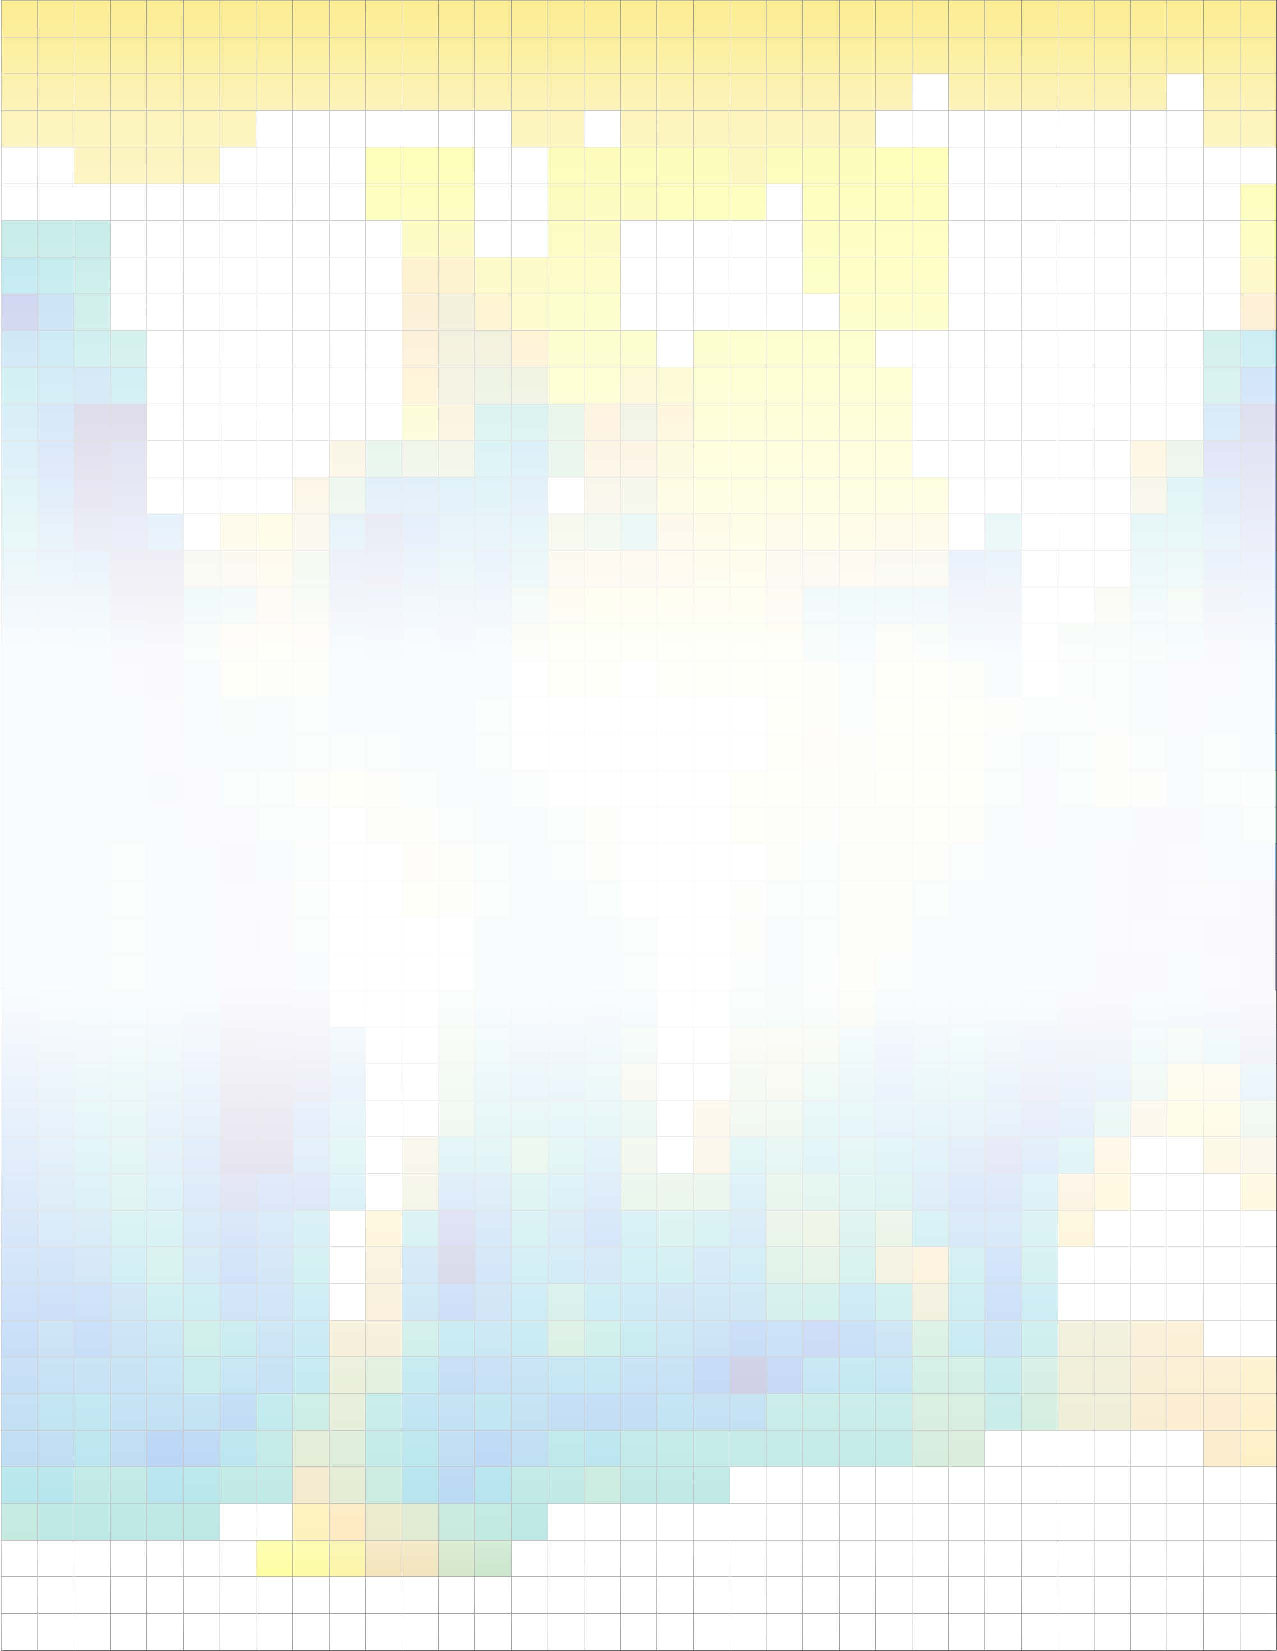
\includegraphics[scale=1]{cover}}} % Image background
\centering
\vspace*{9cm}
\par\normalfont\fontsize{35}{35}\sffamily\selectfont
muffingen v0.3 manual\par % Book title
\vspace*{1cm}
{\Huge Andy Ridgwell}\par % Author name
\endgroup

%----------------------------------------------------------------------------------------
%       COPYRIGHT PAGE
%----------------------------------------------------------------------------------------

\newpage
~\vfill
\thispagestyle{empty}

\noindent Copyright \copyright\ 2017 Andy Ridgwell\\ % Copyright notice

\noindent \textsc{http://www.seao2.info/mycgenie.html}\\ % URL

\noindent Licensed under the Creative Commons Attribution-NonCommercial 3.0 Unported License (the ``License''). You may not use this file except in compliance with the License. You may obtain a copy of the License at \url{http://creativecommons.org/licenses/by-nc/3.0}. Unless required by applicable law or agreed to in writing, software distributed under the License is distributed on an \textsc{``as is'' basis, without warranties or conditions of any kind}, either express or implied. See the License for the specific language governing permissions and limitations under the License.\\ % License information

\noindent \textit{First printing, March 2017} % Printing/edition date

%----------------------------------------------------------------------------------------
%       TABLE OF CONTENTS
%----------------------------------------------------------------------------------------

\chapterimage{Present_0_Ma.jpg} % Table of contents heading image

\pagestyle{empty} % No headers

\tableofcontents % Print the table of contents itself

\cleardoublepage % Forces the first chapter to start on an odd page so it's on the right

\pagestyle{fancy} % Print headers again

%----------------------------------------------------------------------------------------
%       CHAPTER 1
%----------------------------------------------------------------------------------------

\chapterimage{Eocene_50_Ma.jpg} % Chapter heading image

\chapter{Overview of muffingen MATLAB software}

\section{Background}\index{Background}

This documentation describes the collection of MATLAB functions -- \texttt{muffingen} --  needed to create all the configuration files (excluding climatic and biogeochemical \textit{forcing} fields) required by the cGENIE Earth system model. \texttt{muffingen} is designed to take the output from a fully coupled GCM, particularly of past climates with different continental configurations, and re-grid the output needed as boundary conditions by cGENIE and save in the appropriate format. However, \texttt{muffingen} can also be used to draw conceptual alternative Earths (in terms of continental configuration), again saving the required cGENIE files in their appropriate formats.

%------------------------------------------------
%------------------------------------------------

\section{A little history}\index{History}

An earlier collection of MATLAB functions for configuring cGENIE was written by Dr. Andrew Yool of NOCS (Southampton, UK). This was  devised with the intention of facilitating the creation of modern configurations of different grid resolutions based on observed data. Grids (configurations) and studies that arose from this are listed in Table 1.1.

\begin{table}[h]
\centering
\begin{tabular}{l l l}
\toprule
\textbf{Treatments} & \textbf{Response 1} & \textbf{Response 2}\\
\midrule
Treatment 1 & 0.0003262 & 0.562 \\
Treatment 2 & 0.0015681 & 0.910 \\
Treatment 3 & 0.0009271 & 0.296 \\
\bottomrule
\end{tabular}
\caption{Table caption}
\end{table}

The original code was subsequently adapted to take GCM output fields (topography, wind stress and wind speed) instead as input (\textit{in lieu} of observations). Added to this was the capability to also generate the gridded bathymetries needed by the sediment model component as well as generate randomized land surface run-off fields. This was used for a variety of past (geological) configurations and studies, summarized in Table 1.2.

\begin{table}[h]
\centering
\begin{tabular}{l l l}
\toprule
\textbf{Treatments} & \textbf{Response 1} & \textbf{Response 2}\\
\midrule
Treatment 1 & 0.0003262 & 0.562 \\
Treatment 2 & 0.0015681 & 0.910 \\
Treatment 3 & 0.0009271 & 0.296 \\
\bottomrule
\end{tabular}
\caption{Table caption}
\end{table}

However, there were a number of issues with the original collection of MATLAB functions, particularly surrounding the absence of any comprehensive documentation or instructions for use. For instance, users needed to know what constitutes an `island' in the model grid, as well as the rules governing how many island paths to create. The identification of islands and the drawing of island paths needed to be done manually in the MATLAB configuration generator because of difficulties in automatically identifying these unambiguously. This created very significant potential for mistakes and moreover, mistakes that could lead to a climate and ocean circulation being generated, but one in which ocean circulation may not have been solved numerically everywhere. Without carefully checking, there was a very real danger of the situation going unrecognised and any subsequent study would have been rendered invalid.

By default, significant manual clean-up of the land-sea mask and filtering of the bathymetry was also needed. Failure to do this could result in the appearance of biogeochemical `hotspots' on the ocean floor (when nutrients and other tracers become effectively trapped in single cell depressions). However, the clean-up process, particularly with respect to the land-sea mask, lent itself to paleo configurations becoming somewhat subjective, and not only inconsistent between paleo time-slices created by the same user, but between users.

A few issues also existed with the inability to apply land-sea masks in re-gridding wind stress fields. This resulted in high wind stresses over coastal areas becoming entrained in the re-gridded averages generated for cGENIE.

Finally, as the original author has long since ceased to be involved with it, the code had become somewhat difficult to maintain and revise. The lack of documentation also meant that training in using the MATLAB configuration generator became by word-of-mouth.

%------------------------------------------------
%------------------------------------------------

\section{muffingen.m}\index{muffingen}

The intention in creating a new configuration generator was never to re-write the MATLAB code in its entirety, but that is what happened in the end (largely for the aforementioned reasons of the original code being completely unsupported). [exceptions to code being all new]

The principals remain the same. [SUMMERIZE/OUTLINE STEPS]


%------------------------------------------------

\subsection{muffingen code location}\index{CodeLocation}

The current version of the \texttt{muffingen} code can be found on the University of Bristol subversion code repository along with the cGENIE code, e.g.:
\vspace{-5pt}\begin{verbatim}
svn co https://svn.ggy.bris.ac.uk/subversion/genie/branches/cgenie.muffin
--username=genie-user cgenie.muffin
\end{verbatim}\vspace{-5pt}
for the `head' (current development version)\footnote{All this must be typed continuously on ONE LINE, with a S P A C E before `\texttt{--username}', and before `\texttt{cgenie}'.}.
Unless you have logged onto the \texttt{svn} server before from your computing account, you be asked for a password -- it is \texttt{g3n1e-user}.
\\Within the code tree, the primary MATLAB muffinget function lives in \texttt{genie-matlab/muffingen}, with the bulk of the assoctaed functions residing in the \texttt{source} subdirectory of this. 

%------------------------------------------------

\subsection{Examples}\index{Examples}

%%%

%------------------------------------------------

\subsection{About this document}\index{About}

%%%

For problems and issue etc -- see FAQ.

This document lives in LOCATION and can be generatedf from the latex source provided.

Note that in this manual, the paleo configuration images come from 
Ulrich Wieneke, Han Stoutjesdijk, Philippe Simonet \& Virgilio Liverani (Eds.), Gastropoda Stromboidea. URL: http://www.stromboidea.de/ (accessed: August 13, 2007, 16:13)

%----------------------------------------------------------------------------------------
%       CHAPTER 2
%----------------------------------------------------------------------------------------

\chapterimage{Middle_Jurassic_170_Ma.jpg} % Chapter heading image

\chapter{Basic usage}

%------------------------------------------------
%------------------------------------------------

\section{Summary}\index{Summary}

To use the \texttt{muffingen} GENIE configuration generator: at the command line in MATLAB, simply type:

\texttt{>> muffingen(`muffingen\_settings\_*');}

\noindent where \texttt{muffingen\_settings\_*} is the name of an ASCII format configuration file (having a \texttt{.m} filename extension) specifying the required settings (see next section). The generator then starts and depending on the specific settings in the configuration file, may require no user input, or may require user input, either because this option was requested, or because a re-gridding issue arose that requires manual intervention to resolve. A series of plots are created (and saved) as the configuration generation progresses together with the GENIE configuration files themselves. All the various steps plus details of how the contents of the configuration files are generated are reported at the command line, and saved in a n ASCII format \texttt{*.log} file for future reference.

Depending on the configuration file settings, muffingen has 4 main modes of operation which are summarized as follows (and described in more detail, along with specific examples, below):

\begin{enumerate}[noitemsep]
\setlength{\itemindent}{.2in}
\setcounter{enumi}{0}
\item \textbf{Configuration derivation based on re-gridding from a GCM.}
\\ The most common usage of muffingen, enabling a new (typically paleo) configuration to be derived from the output of a GCM experiment. Currently options for utilizing 2 different GCMs are provided: HadCM3 and FOAM.
\item \textbf{Derivation based on an existing topography (`\texttt{.k1}') file.}
\\ Allowing an existing topography to be re-created, or adapted/altered. 
\item \textbf{Derivation based on a prescribed land-sea mask.}
\\ This option will create a configuration from any specified land-sea mask, whether `real' or completely hypothetical. 
\item \textbf{From a blank (all ocean) initial template.}
\\ Finally, this option enables a topography to be `drawn' within muffingen and hence represents an alternative to (3).
\end{enumerate} 

%------------------------------------------------
%------------------------------------------------

\section{The Configuration File}\index{The Configuration File}

When muffingen is run, a configuration file with a specified filename -- the single parameter passed to muffingen when it is invoked at the command line -- is loaded. The configuration file is a plain text (ASCII) format, but is given a .m extension, enabling the values of a number of controlling parameter values to be set.\footnote{Note that the parameter filename is passed as a string without the .m extension (which is implicitly assumed). An error message will be generated if the file does not exist or has the incorrect extension.} The configuration file parameter control facets of muffingen behavior such as the primary model of operation, input and output filenames, what types of configuration files to generate, as well as a number of parameters controlling the finder details of re-gridding and configuration file generation, including whether to enable user-input or not.

The full list of parameter options is summarized in TABLE with the various categories of parameters are summarized in more detail in the sub-sections that follow. Complete descriptions of parameter behavior and usage are given as part of the examples detailed in this, as well as the subsequent Section.

%------------------------------------------------

\subsection{EXPERIMENT INPUT AND OUTPUT}\index{settings1}

These parameters determine input and output, filenames and directories, including the all-important selection of the primary mode of operation.

%------------------------------------------------

\subsection{GRID RESOLUTION \& RE-GRIDDING CONTROLS}\index{settings2}

The first set of parameters in this section control the resolution of the GENIE grid that is created, in terms of the number of cells in longitude, and latitude, as well as the number of depth levels in the ocean. Also provided are parameters to control the maximum ocean depth allowed (i.e. the depth of the base of the bottom-most (\texttt{k=1}) ocean level) and whether the latitude grid is divided into equal increments (common in GCMs) or is equally spaced in sine of latitude, giving an equal-area grid (the default and common GENIE option). Further parameters control several refinements to the grid, including at what longitude the GENIE grid starts (the historical default is -260oE), whether to allow regions of the ocean that are only a single depth level deep, how a higher resolution (GCM) land-sea mask grid is converted into a lower result grid (i.e. what proportion of `land' at higher resolution becomes land in the derived GENIE grid), plus options for controlling the derivation of the sediment grid (for the module SEDGEM), if requested.

%------------------------------------------------

\subsection{OPTIONS -- MAIN}\index{settings3}

This category of options currently only comprises 2 parameters -- one to specify a full set of (common) re-gridding options (over-riding the settings of various indiviaul choices) and one to require user-intervention or not. To automate the creation of GENIE configurations, user-intevention (opt\_user) must be set to \texttt{false}.\footnote{Note that setting \texttt{opt\_user=true} does not a priori guarantee that user-invention is not required (depending on whether an issue arises with the calculation of the \textit{paths} -- see later).}

%------------------------------------------------

\subsection{OPTIONS -- OTHER}\index{settings4}

%%%
%
%------------------------------------------------

\subsection{GRID FILTERING}\index{settings5}

%------------------------------------------------

\subsection{ENVIRONMENT SETTINGS}\index{settings5}

Here ... nothing should typically be altered. par\_dpath\_source sets the relative path to the MATLAB source code for muffingen (excepting the main muffingen.m file) and it is vanishingly unlikely that you would want to place the source anywhere else. The final option is to report further ('debugging') output, such as [WHAT???].

%------------------------------------------------
%------------------------------------------------

\section{Example usage}\index{examples}

The sequence of events\footnote{As per the command line output and also saved in the *.log file.}\footnote{The numbering here is as per the numbered sequence reported by muffingen.} performed by muffingen in this Example is as follows:

\begin{enumerate}[noitemsep]
\setlength{\itemindent}{.2in}
\setcounter{enumi}{0}
\item 
\end{enumerate}

Refinements to this basic Example usage might include consideration/alteration of any or all of the following.

%------------------------------------------------

\subsection{Grid resolution}\index{grid}

%%%

%------------------------------------------------

\subsection{Land area conservation}\index{land}

%%%

%------------------------------------------------
%------------------------------------------------

\section{Interactive Use}\index{Interactive}

Finally, 



%----------------------------------------------------------------------------------------
%       CHAPTER 3
%----------------------------------------------------------------------------------------

\chapterimage{280Marect.jpg} % Chapter heading image

\chapter{Advanced/further usage}

This chapter outlines more advanced usages of the \textsf{muffingen} cGENIE configuration generator. Additional and more minor details regarding further usage can be found in the FAQ Chapter.  

%------------------------------------------------
%------------------------------------------------

\section{Creating hypothetical Worlds}\index{Worlds}

%------------------------------------------------
%------------------------------------------------

\section{Sediment Grids}\index{Sediments}

%------------------------------------------------
%------------------------------------------------

\section{Run-off}\index{Run-off}

%------------------------------------------------
%------------------------------------------------

\section{Albedo}\index{Albedo}




%----------------------------------------------------------------------------------------
%       CHAPTER 4
%----------------------------------------------------------------------------------------

\chapterimage{280Marect.jpg} % Chapter heading image

\chapter{FAQ}

FAQ!

%------------------------------------------------
%------------------------------------------------

\section{Why doesn't it work?}\index{debugging}



* try changing the value of the longitude offset parameter:
  par\_lon\_off
  if having trouble

* lakes cn cause trouble ... ideally you would nto have any -- either ensure they are connected to the open ocena,
    or increase the value of the lake-removing parameter:
    par\_min\_oceann
    (which is the maximum number of grid cells accupied by a lake that will be removed)
    
* The parameter 
  par\_A\_frac\_threshold
  controls what fraction of re-gridded GCM land is considered 'land' in GENIE (the re-gridded land-sea mask)
  A value of 0.5 preserves the approx fractional land area during re-gridding ...
  *except*, subsequent filtering, particularly the filling in of single cell wide channels and lakes,
  increases the re-gridded land fraction. Hence a value less than 0.5 might be suitable.
  Some trial-and-error can come up with a value that preserves global land fraction.



%----------------------------------------------------------------------------------------
%       INDEX
%----------------------------------------------------------------------------------------

\cleardoublepage
\phantomsection
\setlength{\columnsep}{0.75cm}
\addcontentsline{toc}{chapter}{\textcolor{ocre}{Index}}
\printindex

%----------------------------------------------------------------------------------------

\end{document}
